\section{The assessment rubrics}


We classify codes along five different metrics:

\begin{enumerate}
  \item Inter node,
  \item intra node,
  \item core performance,
  \item GPUs, and
  \item input/output.
\end{enumerate}

\noindent
For each of these rubrics, we initially aim for a single three-valued:
All is fine (green), there might be issues (yellow) or there are obvious flaws (red).
In line with our overall presentation approach, we use thresholds of 60\% and 80\% to distinguish these classes.
That is, if the GPU performance is somewhere close to 100\%, all is fine.
However, it is drops below 80\%, we flag it as yellow.
Once the metrics we define for GPUs underrun 60\%, we claim that there are definitely major issues.

 \begin{center}
  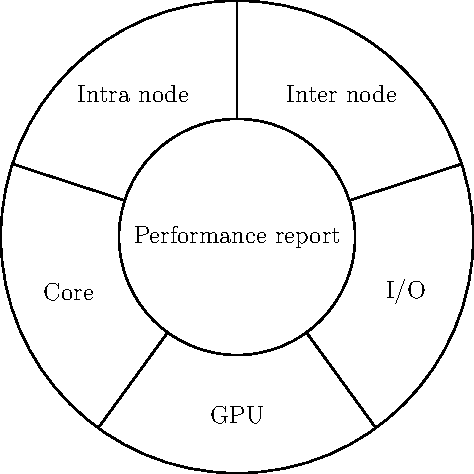
\includegraphics[width=0.55\textwidth]{high-level/performance_diag.pdf}
 \end{center}


\noindent
The idea to look at the five different performance dimensions separatedly is natural yet does not come along without shortcomings.
Many performance issues within a code affect multiple dimensions.
Think about a poor GPU utilisation that materialises in bad load balancing as well.
When we dig down recursively into finer and finer metrics later on, we have to take such cross-influence into account.
Eventually, we might have to return to our highest level of assessment again and again.


As we analyse the dimensions of performance characteristics independently, the order does not really make a difference.
In theory.
In practice, we have to start somewhere.
I personally made the experience that \ldots

%  that it is usually favourable to start with the node-level analysis (intra-node): 
% If the individual cores are not used properly, MPI often does not make that much of a difference and we struggle to keep GPUs busy.
% Often, the next dimension is naturally identified once we look at the node-level performance, i.e.~it tells us what to analyse next.




\paragraph*{How it works}

\begin{itemize}[noitemsep]
  \item[$\boxplus$] Pair debugging is great if people from different disciplines sit together and study the same code.
\end{itemize}


\paragraph*{How it does not work}

\begin{itemize}[noitemsep]
  \item[$\boxminus$] Pair debugging is not good if it transitions into pair programming (``just let me briefly fix this in the code'').
  \item[$\boxminus$] Pair debugging is dangerous if it replaces good architecture and documentation and becomes a knowledge transfer mechanism.
\end{itemize}



\section{Preparation}
\label{section:performance-assessment:preparation}

Before we start a performance assessment, we need to agree on what type of measurements to perform:

\begin{itemize}
  \item There has to be one well-defined benchmark. If we are given a set of
    setups and try to compare them, this will make our task complicated. We run
    risk to compare different characteristics produced by different code parts.
  \item This one benchmark has to run without any user interaction. In the
    normal case, the sponsor has to provide a script which builds and runs the
    whole benchmark ``as a black-box''.
  \item It has to be very easy to scale that benchmark up and down, i.e.~to make the problem solved slightly bigger or smaller. 
  \item The benchmark has to be a simulation run which is representative of a real-world run.
  \item The benchmark does not run for too long, and it does not terminate too early. ``Good'' runs are often 3--5 minutes
    long, so we get a good coverage of performance characteristics, but we do not wait for ages. 
  \item The benchmark has to represent performance characteristics.
\end{itemize}

\noindent
None of the properties are surprising:
We need a well-defined toy setup, and we have to be able to modify its size to make statements on its scalability.
In this context, it is important that we know exactly how changes of input sizes affect the compute workload:
We have to know or have to be told the computational complexity of the underlying algorithms. 
If we have a pure Monte Carlo setup, then doing 100 times more trials should last around 100 times longer.
If we have a parabolic PDE solver with explicit time stepping and a regular grid, we have to know that the problem sizes increases by a factor of $2^d$ if we half the mesh spacing. 
However, these algorithms also have to reduce the time step size, so if we measure over a fixed time span, we actually will have four times more time steps and therefore increase the workload by a factor of $2^{d+2}$ once we half the mesh size.
Finally, if we run an adaptive AMR code for a hyperbolic setup with explicit time stepping or an SPH code, we need some kind of output that tells us exactly how many particles or mesh cells we have and what time step sizes we have picked. In this case, time step sizes go down linearly with mesh spacing.
At the end of the day, we are interested in the \emph{throughput} of the system, i.e.~the time we need to update one quantity of interest.
It is this metric that we will start from in the next steps. 


However, if domain experts tell us afterwards, i.e.~after we have completed our assessment---they will always do that afterwards
    when they are unhappy with the outcome---that this particular run is not
    characteristic for larger runs, as it leaks a feature or does not really use a particular routine
    heavily, our whole assessment exercise if corrupted.
And it the whole assessment will be a big disappointment. 
It is their job to pick a setup that represents what we are interested in and is nevertheless reasonably small.


Having a ``small'' setup that completes in reasonable time is important since some performance analysis
    tools induce significant overheads, i.e.~make the code significantly slower.
    If our vanilla run already needs more than an hour, we will never get an
    answer on time. Furthermore, a lot of tools gather significant amounts of
    data per second. Long-running simulations thus run risk that our analysis
    tools fail to handle the amount of data collected.


No matter how we create this setup, we have to be able to run all experiments with absolutely minimal user interaction (cmp.~Section~\ref{section:behaviour:automate}).
If we have to run through a complex pipeline for each individual experiment, we will not be able to measure anything productively.
In this context, it is important that there's no I/O.
We don't want to study complex outputs; we are busy enough with handling the output of performance analysis tools.

\begin{assessmentcrime}
 The code writes I/O information excessively. 
\end{assessmentcrime}

\noindent
More importantly, if our code writes excessive amounts of data, we
    almost certainly profile the I/O efficiency rather than the runtime
    behaviour. Unless we want to explicitly study I/O, we are well-advised to
    switch off any file outputs, database outputs, but also excessive file
    reads.
 A log file alone can become problematic when these files become suddenly huge or are updated frequently.
 In the best case, a performance assessment benchmark writes and reads barely any data at all, i.e.~it largely hard-coded and silent.

\section{Team dynamics}

Reporting on performance can be a thorny task: 
A successful assessment will allow the reader to make conclusions where and why
and what performance improvements would be beneficial to the code. When we write the report, it
is therefore important to stick to a factual, constructive language: Scientists
tend to be defensive when it comes to their code and often will start to explain why their particular code
has to behave this and that way.



These quickly become non-constructive conversations.
They are tiring and can lead to situations where we don't get the appreciation
for the work invested in the performance assessment.
Potential lessons learned are not taken on board. 
A performance assessment is simply a report how good an algorithm exploits a
machine for one particular setup, and this has to come across in any statement
on the code.
There should be little room to challenge the assessment, and this is best
achieved with a very factual, technical language.

\input{./performance-assessment-intra-node}
\input{./performance-assessment-inter-node}
\input{./performance-assessment-core}
\input{./performance-assessment-gpu} 

\section{Old stuff---do not read}

\section{Performance crimes}


I have made good experiences with starting with a very high-level definition of
\emph{performance crimes}, i.e.~things that are to be blamed for bad
performance:

\begin{enumerate}
  \item The work is unfairly distributed.
  \item We move too much data around. 
  \item Our code does not use the machine features properly.
\end{enumerate}


\noindent
Each crime can be phrased more precisely over the four machine parts
(Figure~\ref{figure:performance-assessment:machine-parts}).
It is important that this does not mean that we look at a crime in an isolated
fashion: A poor work distribution on a node often leads to a poor load
distribution between nodes, too.
We look at the crime and evaluate over all machine parts appropriate.
If the crime arises for a single machine part, we should dig into it.
For this, we again might have to take the whole machine into account and not
only the part where we found it. 



\section{Crime \#1: Unfair work distribution}

Unfair, imbalanced work distribution will manifest in some kind of idling.
Some compute resources will have to wait for others.
This idling might not be idling in a technical sense.
Notably when components poll another component for ``are you done'', they do not
appear to idle. 
However, they are not productive, i.e.~idle in logical sense.




\section{Crime \#2: Too much data movement}

There are different ways to obtain an estimate for or measurements of data
movements.
I do recommend to use monitoring tools.
In line with the previous section, we have too much data movements if the
normalised metric for one of the four machine parts exceeds our threshold. 

\paragraph*{Inter-node}

In-between nodes, the bandwidth of the interconnects is the speed of light: If
we shovel more data from one node to another than the network can cope, we have
an issue.
Without loss of generality, we refer to message passing (MPI) when we speak
about the realisation of inter-node data transfer from hereon.


There are multiple benchmarks on the table to measure the bandwidth of
a system. 
A reasonable one is the ``effective bandwidth"
benchmark \cite{Rabenseifner:2024:EffectiveMPIBandwidth}.
It yields our speed of light quantity $sol_{\text{inter-node}}$.


We can then measure the real bandwidth our simulation obtains from the network. 
Again, there are different tools to measure this. 
Intel's performance snapshot tool is one way.
We combine the measured bandwidth $bw_{\text{inter-node}}$ with the theoretical
one into one metric as

\begin{equation}
m^{\text{(data mov)}}_{\text{inter-node}} = \frac{bw_{\text{inter-node}} }{
sol_{\text{inter-node}} } \leq 0.8.
  \label{equation:performance-assessment:mpi-bandwidth}
\end{equation}


\noindent
A data movement crime is observed if the metric violates this constraint,
i.e.~if we use more than 80\% of the available bandwidth.


\paragraph*{Intra-node}

On current HPC architectures, the cores of a node share their memory. 
Too much data movement hence materialises in high traffic between the last level
cache and the main memory.
It is the memory bandwidth which defines the speed of light inside a node.


The mainstream way to quantify the memory bandwidth is the Stream TRIAD
benchmark \cite{McCalpin:2024:Stream}.
When you build it, ensure that the problem size is large enough to exceed our
last level cache (typically level 3), and that you employ all cores, i.e.~all
cores stress the memory subsystem. 
Stream provides OpenMP support for this.


The actual bandwidth used by your code can directly be measured via performance
counters on modern chips. 
There is a standard interface, PAPI, that allows you to read out these counters,
but the counter semantics can change from machine to machine and machine
generation to machine generation.
They also provide only low-level metrics.
It is more convenient to use a tool such as Likwid \cite{Treibig:2024:Likwid} to
obtain the quantities of interest.
In this case, the metric is memory bandwidth.

We end up with the metric

\begin{equation}
m^{\text{(data mov)}}_{\text{intra-node}} = \frac{bw_{\text{mem bw}} }{
sol_{\text{mem bw}} } \leq 0.8.
  \label{equation:performance-assessment:memory-bandwidth}
\end{equation}



\paragraph*{Core}

Cores typically have their own set of caches, while they share some caches with
the other cores. 
The metric of interest here are therefore the cache hits into the last cache
which is still core-local.
This depends on the system, but most system today have a shared level 3 cache
and a level 2 cache per core.


The level 3 cache mitigates bandwidth penalties arising from memory accesses
(see previous metric), while the level 2 mainly ensures that cores don't
interfere with each other too much.
We hence use the level 2 cache misses as metric to identify core problems:
If less than 80\% of your level 2 cache accesses cannot be served by this cache
(cache misses), we flag this as a performance crime.


\paragraph*{GPU}

GPUs are designed to stream a lot of data through their processing units at
comparatively low cost.
Naturally, you can stress the interconnects between the GPU's processing units
and its memory and hence stop the GPU from unfolding its potential, but this is
not the type of performance crime that we are interested at this point, where
we work more high level.


In a first step, we focus on data movements to and from the GPU, or, on modern
superchips with integrated memory, the access of non-local (host) memory by the
accelerator.
To track the data transfers, tools such as NSight-Systems can provide valuable
insight. 
However, simple runtime profiling is sufficient, as it is, on NVidia hardware,
enabled by setting \texttt{NVCOMPILER\_ACC\_TIME=1}.


For the crime, we relate the data transfer time per kernel
$t_{\text{cpu}\leftrightarrow \text{gpu}}$ to the total kernel execution time
$t_{\texttt{gpu}}$:

\[
  m^{\text{(data mov)}}_{\text{gpu}} = \frac{t_{\text{cpu}\leftrightarrow
  \text{gpu}}}{t_{\texttt{gpu}}} \leq 0.2,
\]

\noindent
defines the constraint that we don't want to violate.
If we do, we consider this to be a performance crime.


\section{Crime \#3: Inappropriate hardware feature usage}


\paragraph*{Inter-node}

Our data movement crime has put an exclusive focus on bandwidth.
The second major characteristics of a network is its latency.
Latency penalties arise from too many small messages.
An algorithmic latency arises from too many messages that arrive unexpectedly,
such that the software side has to invest a lot of cycles to match messages.
This list is not comprehensive.


It is not easy to identify such issues in a black-box manner, i.e.~without
digging into the code.
However, we can employ the bandwidth metric
(\ref{equation:performance-assessment:mpi-bandwidth}) once again:

\[
m^{\text{(data mov)}}_{\text{inter-node}} = \frac{bw_{\text{inter-node}} }{
sol_{\text{inter-node}} } \geq 0.2.
\]


\noindent
Previously, we used high bandwidth requirements to flag data movement crimes.
In return, we can define that an effective bandwidth under 20\% hints at a poor
usage of MPI; for whatever reason.


\paragraph*{Intra-node}

Even though we have excluded excessive memory bandwidth usage and poor load
balancing, there are again many potential execution patterns on a node which
lead to poor performance:
Cache clashes are probably the most prominent ones.


\[
m^{\text{(data mov)}}_{\text{intra-node}} = \frac{bw_{\text{mem bw}} }{
sol_{\text{mem bw}} } \geq 0.2.
\]


\noindent
In line with the discussion above and
(\ref{equation:performance-assessment:memory-bandwidth}), we again struggle to dig into those in a black-box fashion.
However, we can once again assume that exploiting less than 20\% of the
potential bandwidth is an indicator that we struggle to use the node
architecture in a way it is means to be used.


\paragraph*{Core}

Processors today support typical instruction sets or classes of instructions.
We are interested in the most aggressive floating-point instructions for our
work: 
In an ideal world, the processor would be busy all the time with handling
computations, and these computations are all piped through the processor's
vector units.

Our speed of light hence is that all floating-point units are from the highest
instruction set type.
On modern processors, this is AVX512.
We can count these instructions either at runtime or statically over the
executable.


Before we devise a metric, we have to calibrate the number of vector
instructions properly.
If our vector width is 8 for example (AVX512 with double precision), we multiply
the number of AVX instructions by eight.
After that, we can divide the result by the number of total instructions.
A value bigger than 80\% indicates that vectorisation has been used
successfully.
Intel's Application Performance Snapshot tool or scripts around PAPI such as
Likwid deliver you the quantities of interest.


It is important to take all instructions into account:
If a code suffers from a lot integer (index) manipulations, we clearly have
committed a crime in the sense of the present metric.
In contrast, relating the number of vector instructions to the runtime is not
helpful, as stalls could arise from poor memory usage.
We have already taken that into account, and should not double count here.




% An 80\% threshold might be too ambitious for this goal.
% The threshold here is something that has to be agreed upon carefully.


\paragraph*{GPU}

On the GPU, we focus on two problematic phenomena when we speak of an
inappropriate usage of the machinery:
register spilling and kernel overhead.
Register spilling occurs if a code fragment needs too many local variables,
cannot hold them in the register, has to swap them out, and consequently fails
to stream the actual computation through the core, as it notably is penalised
from switching between workgroups.
Kernel launch overhead means that the compute kernel does not really fit to the
GPU, i.e.~is too small, too fine granular, and so forth.
Both phenomena manifest in low effective occupancy compared to the theoretical
occupancy on the machine.


Tool such as NSight-Systems allow you to measure the occupancy.
They even normalise the data appropriately.
We aim for an occupancy above 80\%.
Otherwise, we face a hardware usage crime.



\section{Shortcomings of methodology}

Performance crimes only provide a starting point where to search throughout an
in-depth performance analysis. 
While the previous sections break down the metrics over the hardware parts, I
found it useful only to argue about the aggregate metrics per crime:
Moving around too much memory on a node can lead to situations where the
bandwidth over the network is not saturated.
Arguing however that a fix of this intra-node ``crime'' would eliminate the
data movement issues, i.e.~restricting is to a piece of the hardware,
can be premature:
Next, network bandwidth issues might arise.


Another fundamental issue arises from the fact that all crime metrics
are time-averaged. 
They do not take bursts into account: A code might not exploit all bandwidth all the time, but there might
still be phases, where it is totally bandwidth-bound. 
If you recognise temporal patterns, it can be reasonable to break the search for
crimes down into program phases and to argue separately over them.
The length of the phases then provides a natural indicator if a crime is
considered to be serious or a minor one---you can basically work with a weighted
sum over the metrics.


We finally note that some crime flavours are not actually detrimental to
performance:
Data movements per se are nothing problematic on modern hardware, as long as we
can hide the data transfer behind computations.
This is again a temporal dimension to the data, which we struggle to cover with
the high-level metrics here.
We have to take reported crimes with a pinch of salt.


\section{Next steps}

Once you have identified crimes, it is time to start a proper performance
analysis which relates the observations to more in-depth code studies.


For any type of parallel performance, the groups behind the POP review
methodology have developed an extensive set of tools.
Software such as Scalasca can help the performance analyst to dive into the
reason behind poor scalability.
It can spot local and temporal instabilities, distinguish point-to-point from
collective operations, but also unfortunate realisations such as too late or too
early sends and receives.


For the core performance, a lack of AVX instructions for example can result from
many things: 
There might be a lack of compute work, 
data access might be scattered or non-coalesced,
the compiler might decide that switching instruction sets is too expensive, 
and so forth.
Tools such as MAQAO \cite{MAQAO} can provide valuable insight what is happening
under the hood.


When it comes to GPUs, developers are best advised to consult the software stack
of ``their'' vendor. 
However, the analysis tools for parallel performance start to integrate more and
more GPU-capabilities into their software stack.